\subsection{Gyroskop}
Et gyroskop er et elektromekanisk apparat, som anvendes til at måle omdrejninger pr sekund eller vinkelhastighed om egen akse, hvilket kan ses på \figref{fig:gyro}. Enhederne er henholdsvis revolutions per second (RPS) og $^\circ$/sek. Dette kan give information om orienteringen eller navigationen af objektet, som sensoren optager data fra. Hvis et gyroskop eksempelvis drejes én omgang om egen akse i sekundet, vil den registrere en vinkelhastighed på 360 grader pr sekund. \citep{Sparkfun_gyro}
\begin{figure}[H]
	\centering
	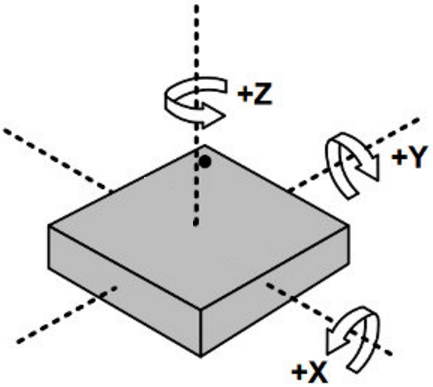
\includegraphics[scale=0.8]{figures/bProblemloesning/gyro.png}
	\caption{På figuren ses et gyroskops måling af rotation omkring egen akse. \citep{Sparkfun_gyro}(Modificeret)}
	\label{fig:gyro}
\end{figure}
Den præcise måde, hvorpå gyroskopet måler på, afhænger af dets type. Der findes blandt andet vibrations, elektrostatiske og kernemagnetisk resonans gyroskoper. \citep{LuingeVeltink2005,TittertonWeston2004} Et gyroskop kan for eksempel registrer vinkelhastighed ved at anvende tyngdekræften og en lille indre masse \citep{Sparkfun_gyro}. Hvis et gyroskop eksempelvis opsamler data undercykling, mens det er placeret proximalt for den laterale malleolus, vil massen blive udsat for en roterende bevægelse omkring en vandret akse. Massen vil blive henholdsvis tungere og lettere i processen på grund af ydre påvirkende kræfter, hvorfor outputtet vil komme til udtryk som en sinus hvis plottet i forhold til tiden. Outputtet er afhængig af tyngdekræftens påvirkning af massen, hvorfor et varierende output kræver en bevægelse. Gyroskopet vil Uanset placering af gyroskopet vil det altså have et fast output, som det vil vende tilbage til efter en bevægelse.\\
%Et gyroskop fungere ved at anvende inerti egenskaberne der opstår når et hjul spindes med en høj hastighed. Ved at hjulet fastholder den samme retning omkring aksen, kan impulsmomentmomentet, dets inertiprodukt samt hastighed være med til at definere en referenceretning. 
%De fundementale principper bag virkningen af et gyroskop er blandt andet det gyroskopiske inerti, som er når hjulet drejer om sin egen akse og står vinkelret på aksen. impulsmomentet som er fordelingen af en masse på et rotor, hvor vinkelhastigheden også har en betydning, og præcession som er rotationen omkring egen akse. 
%De signaler som opfanges af et accelerometrer, inkluderer ikke signaler fra den roterende akse og derfor kan en præcis orientering ikke opfanges. For at forbedre nøjagtigheden, kan man anvende gyroskoper som et supplement til accelerometre .
%Et gyroskop måler vinkelhastighed, hvor ændringen i orientering kan måles ved at integrere vinkelhastigheden på baggrund af en algoritme. \citep{LuingeVeltink2005}
%
\subsection{Sammenligning af accelerometer og gyroskop}
Den væsentligste forskel er, at et gyroskop kan måle rotation, hvilket et accelerometer ikke er i stand til. Accelerometret er fordelagtigt at bruge til at måle orientering af et stationært punkt i forhold til jordens overflade men under bevægelse bliver outputtet mere komplekst. For eksempel vil et accelerometer under frit fald vise 0. \citep{Goodrich2013,LuingeVeltink2005,TittertonWeston2004} \\
Et gyroskop reagerer ikke på vibration eller støj, hvilket et accelerometer kan opsamle som støj på signalet. Derudover reagerer et gyroskop hurtigt men dets output for hældningsvinkel vil blive mere ukorrekt over tid grundet usikkerhed i de enkelte målinger, hvorfor den akkumulerede vinkel ligeledes bliver mere ukorrekt. Et accelerometers respons er langsommere men mere præcis over tid. Igennem kalibrering, hvor hvert apparat assisterer til kalibreringen af den anden, vil de tilsammen kunne holdes korrekt på kort og lang sigt. \citep{Brasca2011,}